\scanpage{5}

\deleted{Considérons les objets suivants}

\deleted{1) $(P,\Delta)$, où $P$ est un groupe abélien libre de rang fini, $\Delta$ une partie finie de $P$, satisfaisant les conditions}

\deleted{a) $\Delta$ engendre $P$}

\deleted{b) Si $a\in\Delta$, $-a\in\Delta$, mais $na\notin\Delta$ si $n\neq1,-1$, $n\in Q$}

\deleted{c) Pour tout $a\in\Delta$, il existe une ``symétrie'' $s_a$ appliquant $a$ sur $-a$, et telle que $s_a(\Delta)\subset\Delta$.}

\deleted{N.B. Alors le $s_a$ en question est unique, \deleted{\unsure{étant un}} en effet \inserted{c'est} l'unique symétrie euclidienne \inserted{dans $PQ$} pour la forme quad. suivante : \deleted{$\unsure{(x,y)}=\unsure{(x',y')}=$} elle se déduit par dualité de la forme}
\deleted{\[
(x,y)=\sum_{a\in\Delta}\langle x,a\rangle\langle y,a\rangle
\quad\text{sur }(PQ)'=(P')Q
\]}
\deleted{On aura alors}
\deleted{\[
s_\alpha x=x-\langle\unsure{\gamma_\alpha|\sigma_\alpha},x\rangle\alpha
\]}
\deleted{pour un $\unsure{\gamma_\alpha|\sigma_\alpha}\in P'Q$ bien déterminé. On montre que l'on a en fait $\unsure{\gamma_\alpha|\sigma_\alpha}\in P'$, i.e. les \deleted{\unsure{c}}}
\deleted{\[
c_{\alpha\beta}=\langle\unsure{\gamma_\alpha|\sigma_\alpha},\beta\rangle
\qquad\text{sont }\in Z
\]}
\deleted{[\uline{provient du} fait que chaque $\alpha$ est indivisible dans $P$, et ceci du fait que $\alpha$ fait partie d'un ``système fondamental de racines'']}
\margin{\figure{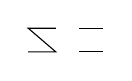
\begin{tikzpicture}\draw(0,.25)--(.35,.25)--(0,.55)--(.35,.55);\draw(.65,.25)--(.95,.25);\draw(.65,.55)--(.95,.55);\end{tikzpicture}}}

\deleted{2) $(P,P',\Delta,\Delta',\varphi)$, où $P,P'$ sont deux groupes abéliens libres de rang fini \deleted{\unsure{en dualité}}, \inserted{\uline{accouplés à $Z$}}, $\Delta\subset P$, $\Delta'\subset P'$, \inserted{$\varphi$ une bijection de $\Delta$ sur $\Delta'$, \deleted{\unsure{avec}}} les conditions suivantes étant vérifiées :}

\deleted{a) $PQ$ et $P'Q$ sont en dualité, $\Delta$ engendre $P$, \inserted{$\Delta'$ engendre $P'$}}

\deleted{b) Pour tout \deleted{$\unsure{\alpha'}\in\Delta'$}\inserted{$\alpha\in\Delta$}, \inserted{tel que $\varphi(\alpha)=\alpha'$, l'endomorphisme}}
\deleted{\diagram{\begin{tikzcd}[ampersand replacement=\&]
s_\alpha:\unsure{\xi|\gamma}\arrow[r,mapsto]\&\unsure{\xi|\gamma}-\langle\alpha',\unsure{\xi|\gamma}\rangle\alpha
\end{tikzcd}}}
\deleted{applique $\Delta$ dans $\Delta$, \deleted{\unsure{ainsi}}}
\margin{\figure{\begin{tikzpicture}\draw[<->](0,0)--(0,.65);\end{tikzpicture}}}

\margin{\inserted{Si $\alpha'=\varphi(\alpha)$, on a $\langle\alpha',\alpha\rangle=2$}\figure{\begin{tikzpicture}\draw(0,0)--(.4,.65);\draw(.4,.65) circle(.04);\end{tikzpicture}}}

\deleted{b') Pour tout $\unsure{\gamma|\xi}\in\Delta'$, $\alpha\in\Delta$ tel que $\varphi(\alpha)=\unsure{\gamma|\xi}$,}
\deleted{\diagram{\begin{tikzcd}[ampersand replacement=\&]
s'_\alpha:\unsure{\xi'|\gamma'}\arrow[r,mapsto]\&\unsure{\xi'|\gamma'}-\langle\unsure{\xi'|\gamma'},\alpha\rangle\alpha'
\end{tikzcd}}}
\deleted{invarie $\Delta'$}

\mspage{4}
